Para que nuestra smartTV sea capaz de usar Miracast sin necesidad de Chromecast necesitaría soportar Wi-Fi Direct, es decir, estuviera conectada por Wi-Fi y fuese compatible con ella.

\begin{figure}[ht] 
	\begin{minipage}[b]{0.55\linewidth}
		La conexión está creada vía Wi-Fi Protected Setup (WPS), mecanismos para facilitar la configuración de una red WLAN con seguridad WPA2.
		WPS contempla cuatro configuraciones para el intercambio de credenciales, PIN (Personal Identification Number), PBC (Push Button Configuration), NFC (Near Field Communications) y USB (Universal Serial Bus). La configuración PIN no es recomendable por su debilidad ante ataques de fuerza bruta.
	\end{minipage}%%
	\begin{minipage}[b]{0.45\linewidth}
		\centering
		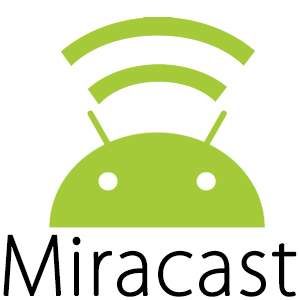
\includegraphics[width=.55\linewidth]{./Imagenes/miracast.jpg} 
	\end{minipage} 
\end{figure}



En la capa de internet es usado IPv4, en la capa de transporte es usado TCP o UDP. En la capa de aplicación el stream es inicializado y controlado por RTSP y RTP.
Los dispositivos que envían y reciben información tienen que estar certificados para Miracast, pero existe un plug para dispositivos no certificados.



\subsubsection{MiracleCast}
MiracleCast es una alternativa de código abierto a Miracast. El nombre, en palabras del autor, viene por que creía que necesitaba un milagro para crear una red Wifi-P2P estable (basado en $wpa_supplicant$), debido a los problemas que había tenido.

El núcleo de MiracleCast es un demonio llamado miracled \cite{MiracleCast}, que controla links locales, las peticiones de conexión, se encarga de
la codificación del protocolo y el parsing.
Su línea de comandos puede ser usada para controlar el demonio, crear nuevas conexiones, modificar parámetros, etc.
Soporta un modo interactivo que muestra las peticiones de conexión y permite al usuario aceptarlas o no.

El código fuente se puede encontrar en \href{https://github.com/albfan/miraclecast}{github}.